\documentclass[UTF8,a4paper,zihao=-4,fontset=fandol]{ctexart}
\usepackage[margin=24mm]{geometry}
\usepackage{amsmath,booktabs,tabularx,graphicx}
\usepackage[hidelinks]{hyperref}
\setlength{\emergencystretch}{2em}
\title{基于深度学习的 Micro-C 接触矩阵处理\\[0.4em]
  \large 深度学习综合实践课程项目报告}
\author{A：hycx233（组长）\quad B：onlysonder\\C：lanshuheng9-oss}
\date{2026 年 9 月 20 日\quad 阶段报告骨架}

\begin{document}
\maketitle
\noindent\textbf{文档状态：}本稿用于分工写作，尚非最终实验报告。
当前填入了数据准备与共享预处理的已验证事实；模型训练及后续分析结果按各节标记补充。
最终提交前补全摘要、正式结果、成员姓名及实际贡献比例，并更新日期。

% 负责人：A / hycx233。各模块的细节由对应负责人补充。
\section{任务目标}
本项目按课程实践方案\cite{course}完成已知结构识别与解释、新结构候选发现、
多轨道可视化三个必做任务，选做不同条件下的结构差异定位。
数据条件统一为 WT、$\Delta stpA$ 和 $\Delta hns\Delta stpA$，每个条件使用两个重复。
已知结构类型为 OPCID、CHIN 和 CHID，定义与实验背景参照原研究\cite{paper}。

\section{设计思路}
\subsection{共享输入与两类分析目标}
已实现共用的矩阵读取、坐标转换、窗口提取和数据划分。
当前把 10 bp 数据聚合至 100 bp，截取 24 kb 窗口并生成 $128\times128$ 模型输入；
是否采用附加视角，应由真实窗口效果决定。
共享数据流程已在六个样本上验证，方法和分组统计见第 3 节；模型效果尚未评价。

强度比较保留测序深度归一化后的接触信号；
形态分析使用按基因组距离计算的观察值与期望值之比（O/E），再作统一的数值变换。
不能用每个窗口独立缩放到相同均值的数据判断不同条件的强弱变化。
环状染色体上的跨起点窗口需要首尾拼接，背景距离也要考虑环状结构。

\subsection{模型与评价路线}
已知结构识别采用轻量 CNN，报告准确率、Macro-F1、混淆矩阵与简单基线，
结合显著性图和失败案例说明模型依据。
候选发现采用小型卷积自编码器，以重建误差打分，使用 PCA 和 DBSCAN 整理候选表征。
候选应与已知结构及随机背景对照，并在独立重复的相同位置检查复现性。
不能仅凭分类器低置信度或聚类噪声标签宣称发现了新结构。

正式划分需使同一结构、其重复和空间重叠的输入不跨训练、验证、测试集合。
模型选择使用验证集，测试结果用于最终评价。
任务四比较两个突变条件相对 WT 的变化，并用 WT 两个重复的差异作参照。
这些规则将在对应实验章节用实际参数、对照和结果落实。

% 负责人：A / hycx233。数据准备与共享预处理的已验证事实。
\section{数据来源与准备}
\subsection{样本与标注}
使用课程提供的 Micro-C 接触矩阵和\texttt{标注数据.xlsx}。
原研究公开数据登记于 GEO 总系列 GSE272161\cite{geo}。
WT 使用 Micro-C 子系列 GSE272159 所列的两个 37\,$^\circ$C 附件\cite{geomicroc}，
突变数据实际输入取自课程提供的 \texttt{GSE272161\_RAW.tar}，
选择性解压 GSM8950761 至 GSM8950764 四个成员。
这四个样本也列于 GSE272159；本项目以课程配套文件为实际输入。
本阶段只读原材料，转换后的标注、基因表和样本表分别保存。

\begin{table}[htbp]
\centering
\caption{已核对的数据准备结果（任务 \#1）}
\begin{tabularx}{\linewidth}{l r X}
\toprule
产物 & 记录数 & 内容 \\
\midrule
结构表 & 344 & OPCID 68 条、CHIN 250 条、CHID 26 条 \\
基因表 & 4,516 & 4,451 个不同名称；保留同名但位置不同的记录 \\
样本表 & 6 & WT、$\Delta stpA$、$\Delta hns\Delta stpA$ 各两个重复 \\
\bottomrule
\end{tabularx}
\end{table}

六个实际矩阵的染色体名均为 \texttt{NC\_000913.3}，长度为 4,641,652 bp，
分辨率为 10 bp，每个样本有 464,166 个 bin；计数为 \texttt{int32}，
采用上三角对称存储，均无预存的 \texttt{weight} 列。
因此共享预处理显式读取原始 counts，不假定平衡权重已经存在。

\subsection{坐标口径与追溯}
下游统一使用染色体名 \texttt{NC\_000913.3} 和 0-based 左闭右开区间。
Excel 中的 \texttt{MG1655} 作为同一染色体的别名。

Table 1 的基因坐标与 NCBI 的 1-based 闭区间一致，转换时仅起点减一，终点和链方向不变。
例如 \textit{thrL} 的源范围为 $190\ldots255$，转换后为 $[189,255)$；
\textit{hns} 的源范围为 $1292509\ldots1292922$，转换后为 $[1292508,1292922)$，
仍为负链\cite{thrl,hns}。

结构表沿用作者接触图坐标的数值，不减一。
作者分析代码直接以坐标整除 25 进行分箱\cite{authorcode}。
将课程标注按该规则转为作者的 BED/BEDPE 格式，
68 条 OPCID、250 条 CHIN（区间及中心）、26 条 CHID 均匹配。
原文未明确说明 Excel 结构端点逐碱基的开闭含义，
因此将其解释为 $[start,end)$ 是本项目的统一接口约定。
CHIN 的 Center 复制原始字段，所有记录保留来源工作表、行号与原坐标。

\subsection{数据准备检查}
结构表与基因表已逐行回查 Excel，检查计数、唯一标识、坐标范围、长度和 CHIN 原 Center。
六份矩阵已核对元数据，解压文件可复用，原始矩阵和压缩包不改写。
还在 WT 两个重复中各提取了三类结构的真实窗口，作为初始 CPU 读取与定位预览。
这批初始预览显示统一色标下的 $\log(1+\mathrm{raw\ counts})$，
仅用于核对读取位置，不构成条件差异证据；正式共享输入使用下述归一化。

运行入口为 \path{scripts/prepare_annotations.py}、
\path{scripts/prepare_samples.py} 和 \path{scripts/preview_structures.py}。
详细命令、表字段和代表预览保存在仓库的\texttt{docs/数据准备说明.md}。

\subsection{共享归一化与有效掩码}
采用流式聚合，将原始 10 bp 上三角唯一接触计数相加至 100 bp 工作矩阵，
读取局部窗口时补成对称矩阵，不展开全基因组稠密数组。
令 $C_{ij}$ 为工作矩阵计数，样本总接触量和深度归一化强度分别为
\[
  T=\sum_{i\leq j}C_{ij},\qquad I_{ij}=\frac{10^6 C_{ij}}{T}.
\]
$T$ 对每个接触计数一次；轨道的边缘信号取对称矩阵行和，
非对角计数加到两个端点，对角计数只加一次。
不同条件的强度比较使用 $I$，不把每个窗口独立缩放到同一均值。

有效 bin 要求边缘信号大于零且宽度完整为 100 bp。
对 $n$ 个工作 bin，定义环状距离 $d(i,j)=\min(|i-j|,n-|i-j|)$。
令 $P_d$ 为距离 $d$ 上两个端点都有效的无序 bin 对集合，包含零接触对，
则形态背景、O/E 和统一变换为
\[
  E_d=\frac{\sum_{(i,j)\in P_d}C_{ij}}{|P_d|},\qquad
  R_{ij}=\frac{C_{ij}}{E_{d(i,j)}},\qquad
  F_{ij}=\frac{\log(1+\min(R_{ij},10))}{\log(11)}.
\]
O/E 仅在 $E_d>0$ 且端点有效时计算，形态另掩去主对角线。
强度保留对角并有独立掩码。无效值以零存储，不能据此解释为接触减弱；
在同一位置比较多个样本时，要使用这些样本有效掩码的交集。
全局深度和距离背景不使用结构标签或模型指标，截断值在模型评价前固定。

\subsection{环状窗口与模型输入}
窗口以结构中心为中心，跨度 24 kb。跨起点时按真实基因组长度 $L=4641652$
拆成首尾两段，读取四个矩阵块，保留两段之间的非对角接触。
100 bp bin 与窗口端点不一定对齐，局部矩阵通常有 240--242 格。
生成 $128\times128$ 输入时，以真实 bin 区间与目标格的重叠面积作权重，
只平均有效面积，同时保存模型掩码与有效面积比例。

末尾 52 bp bin 的原始计数保留，但不参与强度及形态统计。
距离背景使用 100 bp 网格上的环状距离近似，跨起点距离最多相差 48 bp；
真实窗口坐标和面积权重仍使用实际 $L$，不会把染色体补长。

\subsection{分组与导出}
对已知结构的完整 24 kb 窗口求环状空间重叠连通分量，
并检查实际读取的 100 bp 边缘 bin。同一分量的结构、重复及后续增强使用同一集合。
固定种子为 20260918，按类别数与总量分配约 70\%/15\%/15\%，不使用模型结果选择划分。
344 条结构形成 59 个分量，最大分量 20 条；没有排除任何已知结构。

\begin{table}[htbp]
\centering
\caption{共享划分：结构位置与 WT 两个重复的输入窗口}
\begin{tabular}{l r r r r r}
\toprule
集合 & OPCID & CHIN & CHID & 位置总数 & 两重复窗口 \\
\midrule
train & 48 & 175 & 18 & 241 & 482 \\
val & 10 & 37 & 4 & 51 & 102 \\
test & 10 & 38 & 4 & 52 & 104 \\
\bottomrule
\end{tabular}
\end{table}

分类导出 688 个输入。另导出 24 个随机背景位置、共 48 个重复窗口，用于发现模块接通入口；
背景位置不与已知结构注释相交，窗口不得连接不同集合，
与已有窗口重叠时继承其集合。六样本检查另有 24 个示例窗口，其中跨起点检查标记为
\texttt{probe}，不参与训练、验证或测试。
背景和跨起点 \texttt{probe} 的标签为 $-1$，不能混入三分类训练。

\subsection{实际运行与验证}
2026 年 9 月 20 日已在 CPU 上用六份真实数据跑通任务 \#2。
首次缓存生成约耗时 253 秒，复用缓存导出窗口及绘图约 23 秒；
这些是本次运行记录，不是其他机器的耗时保证。
九项针对性检查通过，六个样本聚合前后的总计数一致。
WT rep1 的五个普通及首尾窗口另与原始 10 bp 局部像素的独立聚合结果逐元素一致。
跨集合共享的实际 100 bp bin 数为零。
688 个分类输入已由分类 PR \#13 的实际读取代码加载，数组、标签与 CSV 行序一致，
且保留提供的划分；背景与示例输入也通过有限数、对称性、标签、行序和坐标检查。
\textbf{本阶段没有运行模型训练，不报告模型性能。}

安装仓库依赖并准备原始样本后，从仓库根目录执行：
\begin{verbatim}
OPENBLAS_NUM_THREADS=1 python scripts/prepare_data.py
\end{verbatim}
详细方法、验证记录和运行时的代码指纹保存在以下位置：
\begin{flushleft}
\small
方法说明：\texttt{docs/共享预处理说明.md}\\
验证记录：\path{docs/results/preprocessing/validation.json}\\
分组摘要：\path{docs/results/preprocessing/splits.json}\\
运行记录：\path{outputs/preprocessing/default/run_*.json}
\end{flushleft}

% 负责人：B / onlysonder，对应 #3、#4。
\section{已知结构分类与解释}
\textbf{待 B 补充实际方法与结果。}本节目前不报告模型性能。

\subsection{方法与训练设置}
补充 CNN 结构、输入、损失函数、类别不平衡处理、数据划分来源、随机种子、
优化器与训练停止规则，记录正式运行命令和权重位置。
仅描述实际采用的设置，区分小样本试运行与正式实验。

\subsection{分类结果与解释}
从已保存结果填入准确率、Macro-F1、各类表现、混淆矩阵及简单基线对照。
选择三类代表样本和失败案例展示解释图，核对样本属于哪个集合，
说明模型关注区域与结构形态的关系及其局限。

% 负责人：C / lanshuheng9-oss，对应 #5、#6、#7；跨重复结果由 B 补充。
\section{候选结构发现与可视化}
候选并不自动等于新结构。本节所有数值来自 2026 年 9 月 21 日 mask 修订后的正式运行，
完整命令、代码版本和结果表位于 \texttt{docs/results/}。

\subsection{候选发现与聚类}
我们用 WT rep1 中排除已知结构的 17 个训练背景窗口训练 32 维卷积自编码器，
4 个验证窗口选择轮次，3 个测试背景不参与训练或选轮次。逐窗口有效 mask 与上三角
mask 取交集后计算 loss，数据缺口的填零区域不参与训练和打分。模型在第 25 轮取得最佳
验证 masked MSE 0.022307。随后以 1 kb 步长扫描 4,641,652 bp 染色体，共得到
4,642 个 24 kb 窗口，并按重建误差前 1\% 保留 47 个候选。候选召回 21/344
个已知结构（6.1\%）；重建误差与接触强度的 Pearson 和 Spearman 相关分别为
0.828 和 0.765，因此高分明显受到接触密度影响，不能单独作为新结构证据。

候选、已知参考和 200 个固定种子随机背景使用同一编码器与标准化变换；背景从 1,075
个不与任何已知结构重叠的合格位置中抽取，实际重叠数为 0。标准化后保留
10 个白化 PCA 分量，再用 DBSCAN（\texttt{eps=3.0}，
\texttt{min\_samples=5}）聚类。相互重叠的候选窗口先合并，47 个窗口实际只有
10 个独立位置。唯一的非噪声簇包含 297 个已知参考成员；其中 9 个候选来自
4 个独立区域，4 个还直接与已知结构重叠。其余 38 个候选为 DBSCAN 噪声。

本组约定疑似新簇必须同时包含至少 5 个独立候选位置、没有已知参考成员，且候选区间
均不与已知结构重叠；DBSCAN 的 $-1$ 噪声不算簇。本次没有任何簇满足规则，因此不
宣称发现新结构，留待跨重复任务检查全部候选。作为表征检查，306 个无歧义已知参考
位置按完整窗口的空间重叠连通关系分成 60 组，再做 5 折平衡逻辑回归；实测跨折重叠
对数为 0，balanced accuracy 为 0.518，多数类 balanced accuracy 为 0.333，说明
隐向量含有有限类别信息，但不足以替代正式分类器。

\begin{figure}[htbp]
  \centering
  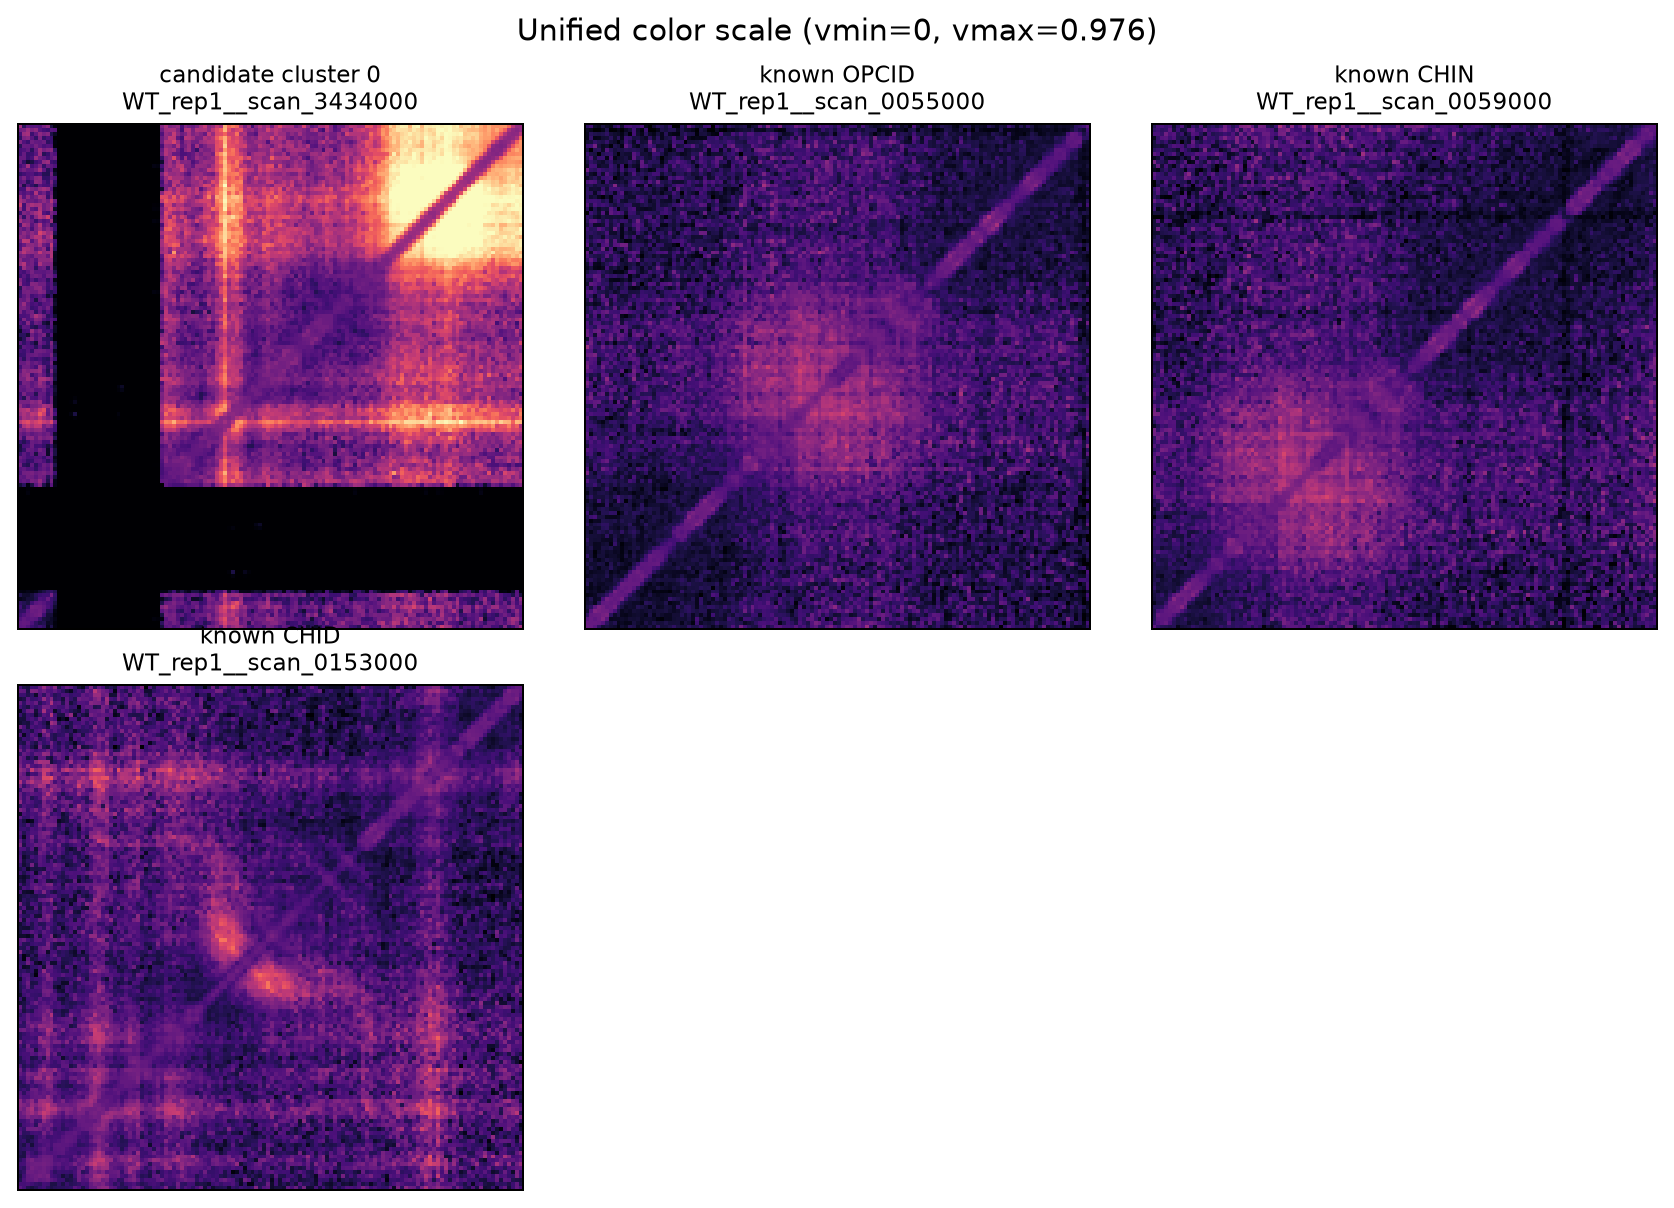
\includegraphics[width=0.92\linewidth]{../results/clustering/cluster_representatives.png}
  \caption{候选簇代表与三类已知结构参考。所有热图统一使用 0--0.816 色标，灰色为无效像素。}
\end{figure}

\subsection{全基因组多轨道图}
轨道信号复用 100 bp 共享缓存：上三角非对角接触累加到两个端点，对角接触只计一次，
再按每个样本的总接触量缩放至每百万，先归一化两个重复再取条件均值。图上使用平方根
显示压缩动态范围，原始保存数组仍是线性归一化信号。

WT、$\Delta stpA$ 和 $\Delta hns\Delta stpA$ 三条件共六个真实重复被绘制为四面板图：
重复曲线及全基因组中位数灰线、条件均值、基因轨道和 CHIN/OPCID 轨道。全基因组按
10 kb 输出 465 张，末图正确覆盖 $[4,640,000,4,641,652)$；最后不足 100 bp 的无效
bin 留白，没有画成假性零值。首图、末图和 4 张代表图均已人工检查，完整图集位于本地
\texttt{outputs/tracks/all/}，可提交的运行记录和代表图位于
\texttt{docs/results/tracks/}。

不同条件下的局部趋势并不一致：$[1{,}210{,}000,1{,}220{,}000)$ 和
$[2{,}480{,}000,2{,}490{,}000)$ 中双突变条件在多数位置高于其他两组，
$[3{,}800{,}000,3{,}810{,}000)$ 则主要表现为 $\Delta stpA$ 信号较高。这些图用于展示
轨道的实际读法与局部差异，不把单个区间的曲线高低当作全基因组显著性结论。

\begin{figure}[htbp]
  \centering
  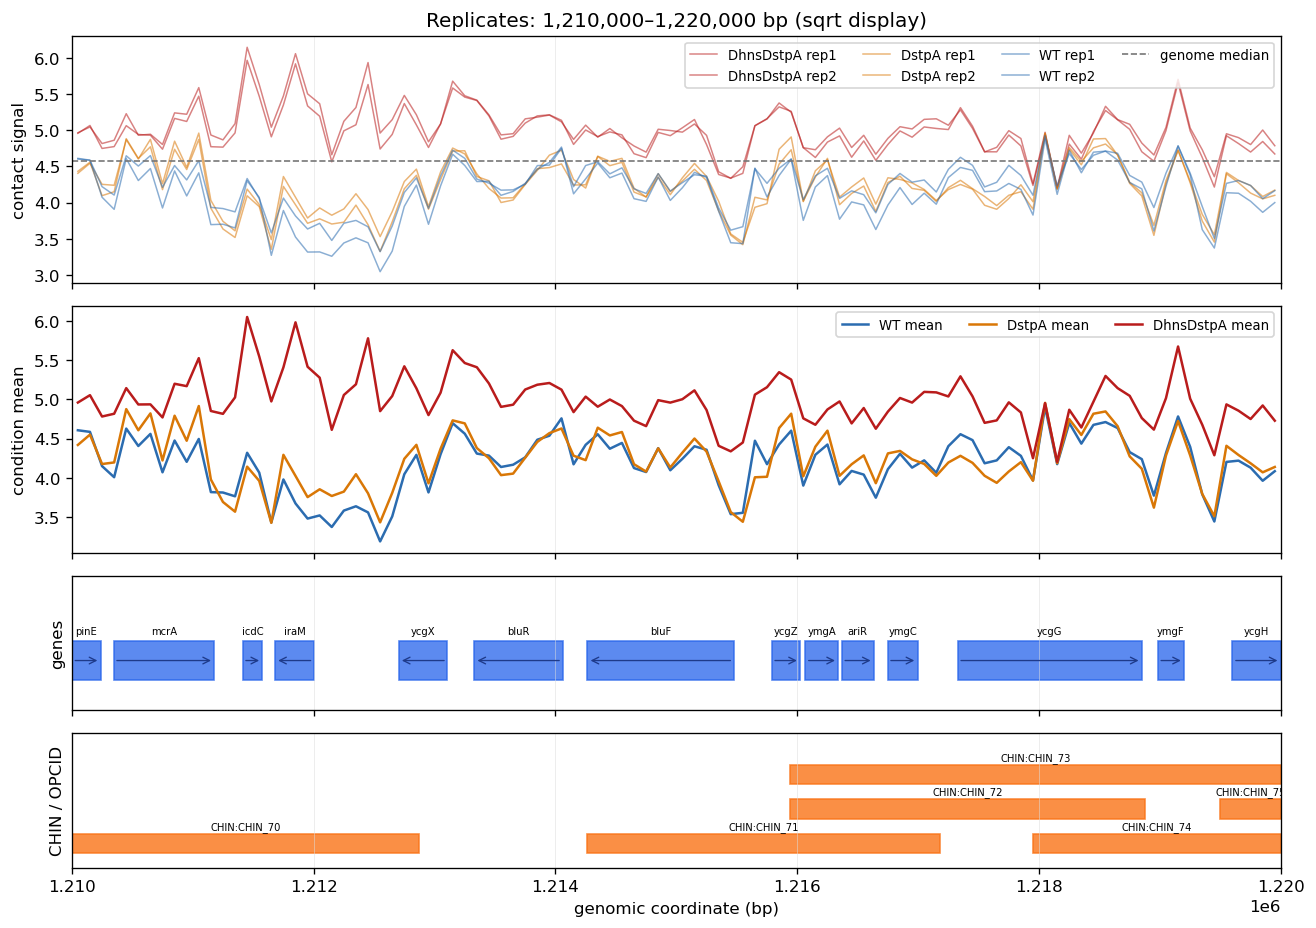
\includegraphics[width=0.96\linewidth]{../results/tracks/tracks_1210000_1220000.png}
  \caption{$[1{,}210{,}000,1{,}220{,}000)$ 的三条件轨道。每个重复先独立归一化，条件均值在线性尺度上计算后再开平方显示。}
\end{figure}

\begin{figure}[htbp]
  \centering
  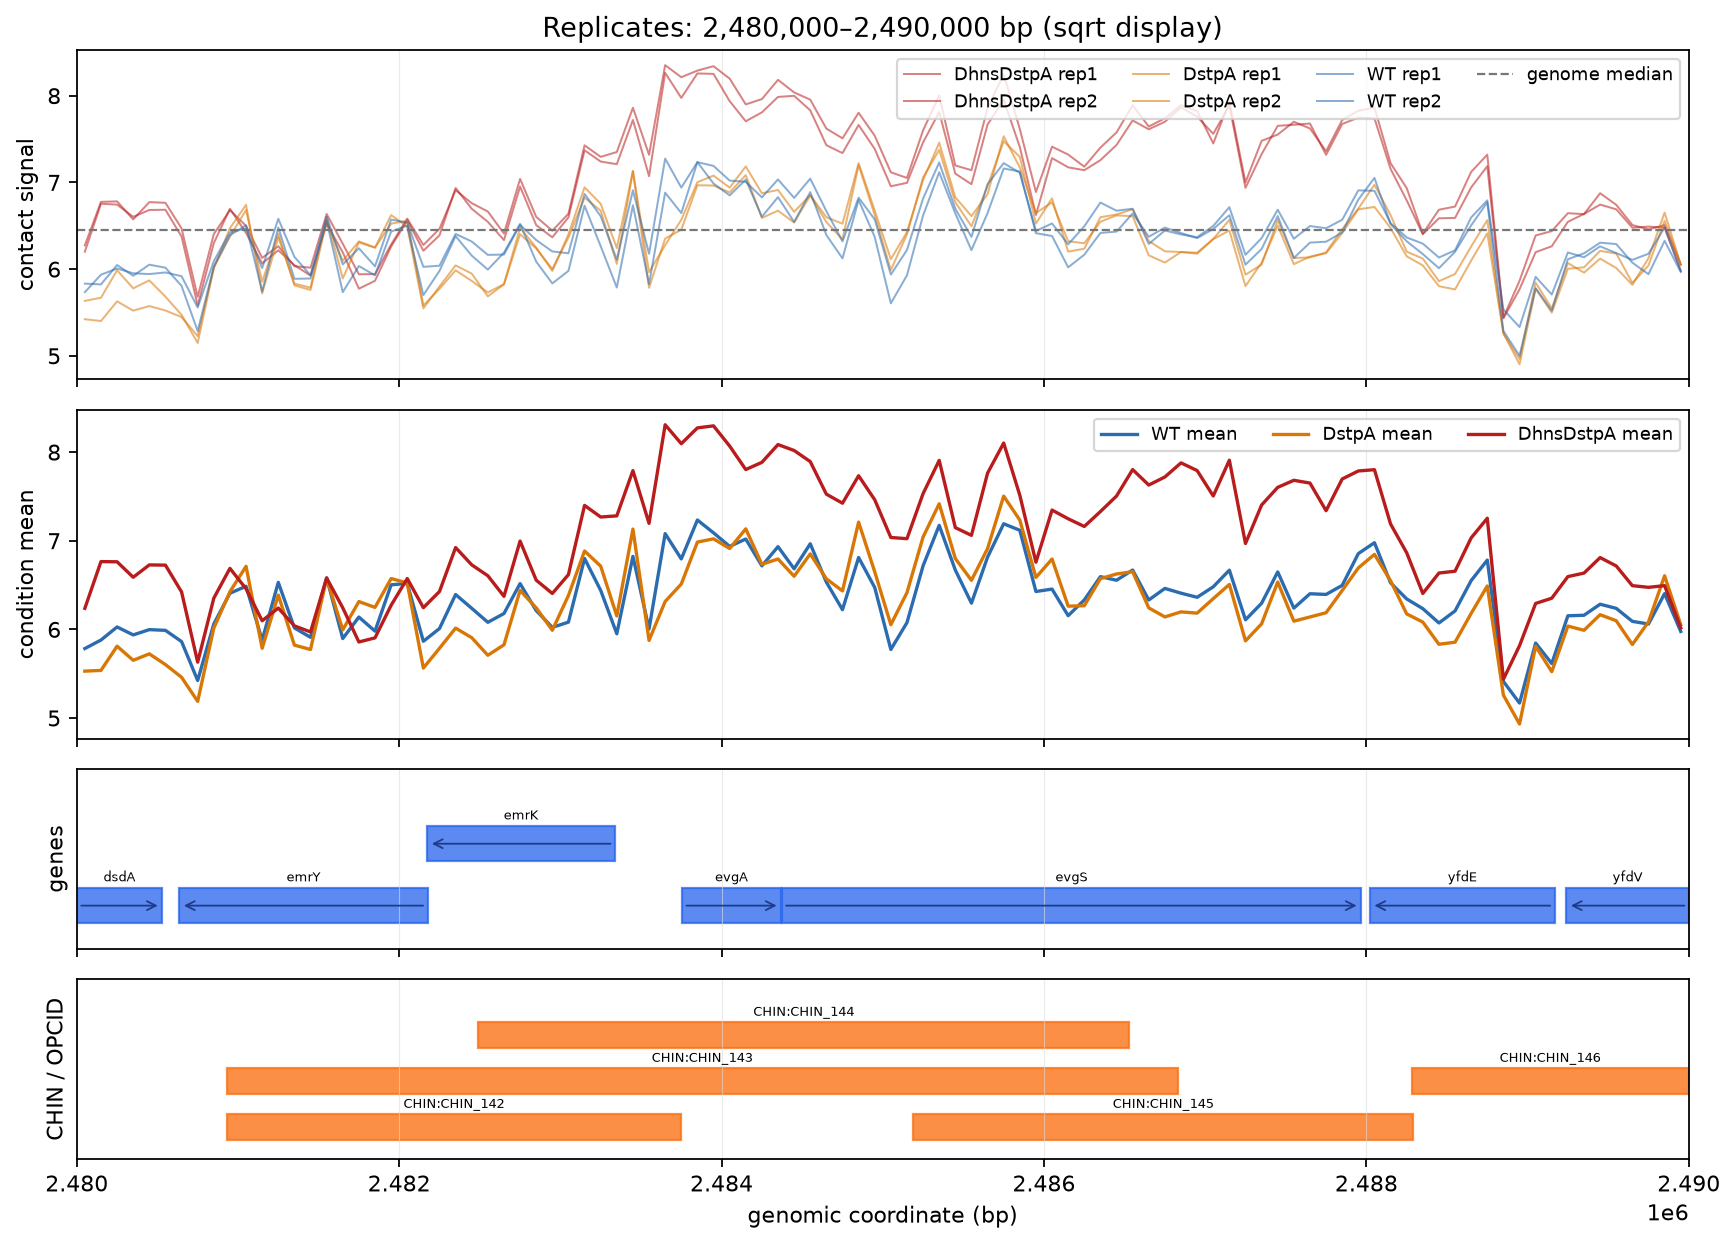
\includegraphics[width=0.96\linewidth]{../results/tracks/tracks_2480000_2490000.png}
  \caption{$[2{,}480{,}000,2{,}490{,}000)$ 的三条件轨道。图中同时保留重复曲线、条件均值、基因与已知结构坐标。}
\end{figure}

\begin{figure}[htbp]
  \centering
  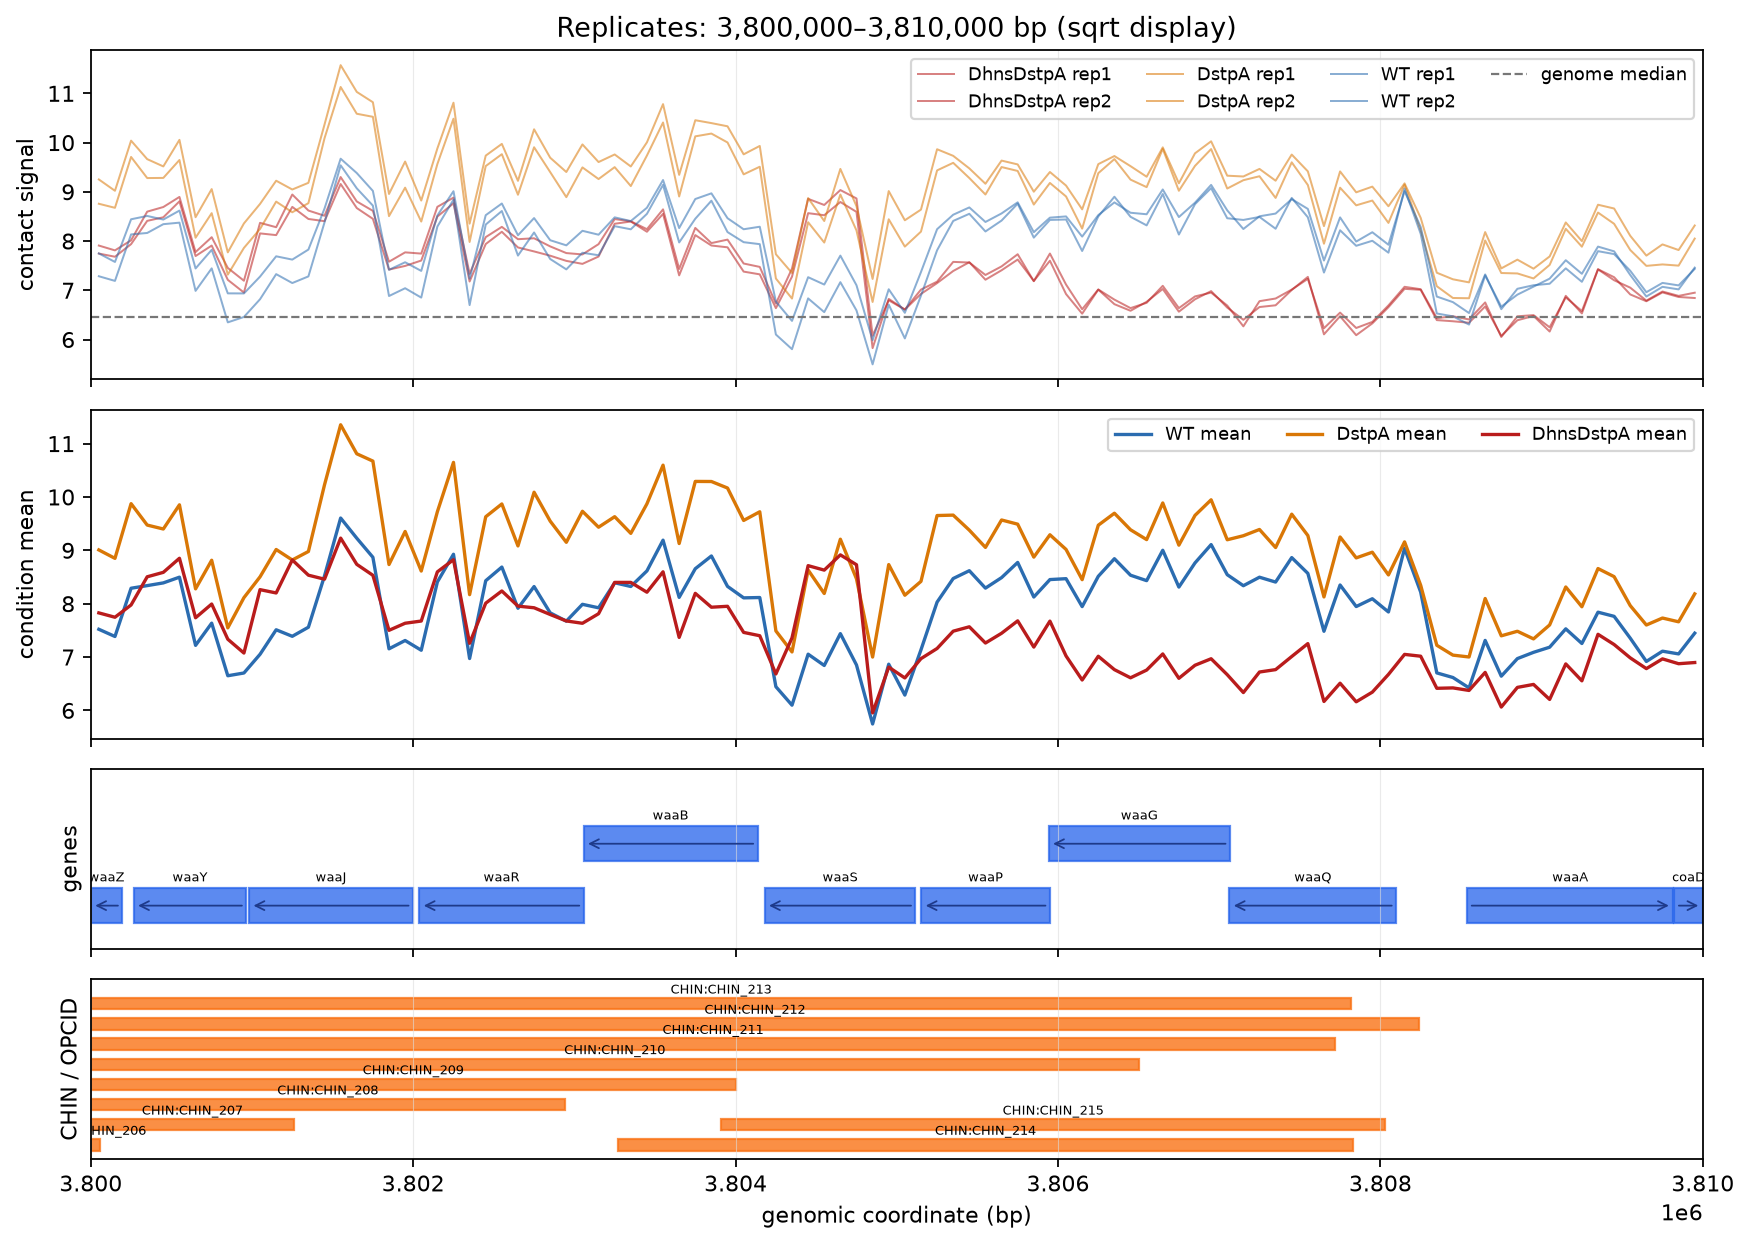
\includegraphics[width=0.96\linewidth]{../results/tracks/tracks_3800000_3810000.png}
  \caption{$[3{,}800{,}000,3{,}810{,}000)$ 的三条件轨道。本区间与前两例呈现不同的条件顺序，说明不应使用单个代表区间概括全基因组。}
\end{figure}

% 负责人：A / hycx233，对应 #8。
\section{不同条件下的结构差异定位}
\textbf{共享预处理已完成，待 A 完成任务 \#8 后补充。}
本节比较 $\Delta stpA$、$\Delta hns\Delta stpA$ 相对 WT 的结构信号变化。
需说明结构内信号汇总方式、深度归一化、伪计数与对数倍数变化的定义，
报告两个重复各自的数值和方向，并以 WT 重复间变化作为参照。

从差异表选择代表案例，给出同尺度的 WT 与突变条件热图及坐标。
结论区分观察到的条件差异与因果解释，
不能把双缺失条件下的全部变化归因于其中一个因子。

% 负责人：B / onlysonder，对应 #9、#12；其他成员提供各自运行记录。
\section{重复验证与复现说明}
\textbf{待 B 补充实际验证记录。}
候选跨重复验证在 WT rep2 的相同位置提取窗口，
对照已知结构和随机背景，说明使用的矩阵、对角线掩码、有效像素与相关性指标。
报告筛选规则如何固定，不把相邻重叠窗口当作多个独立复现证据。

复现说明填写实际软件版本、设备、数据与代码版本、随机种子、运行命令、
权重及结果位置，列出已经在另一环境复跑的代表流程和仍未执行的步骤。
数据准备可在 CPU 上进行；正式模型训练使用什么设备，以实际运行记录为准。

% 负责人：A / hycx233 汇总，三人核对自己的交付与贡献。
\section{讨论与结论}
\textbf{待正式结果齐备后填写。}
总结四个任务实际完成的内容、最有依据的观察以及样本数、类别不平衡、
候选判定和重复一致性等限制。
当前已核对数据准备与共享预处理流程，但没有据此得出模型效果或生物学新发现的结论。

\section{成员分工与贡献}
下表记录计划分工，\textbf{不代表最终实际贡献比例}。
最终根据实际交付由三人共同确认百分比，总和为 100\%。

\begin{table}[htbp]
\centering
\begin{tabularx}{\linewidth}{l X c c}
\toprule
成员 & 主要分工 & 计划份额 & 实际贡献 \\
\midrule
A：hycx233 & 数据准备、共享预处理、差异定位、整合与提交 & 约三分之一 & 待填写 \\
B：onlysonder & 分类与解释、重复验证、复跑与交付打包 & 约三分之一 & 待填写 \\
C：lanshuheng9-oss & 候选发现、聚类、多轨道图与案例 & 约三分之一 & 待填写 \\
\bottomrule
\end{tabularx}
\end{table}

三人分别撰写自己模块的报告章节、演示内容和讲解片段。
演示文稿在结果定稿时统一选择 Beamer 或 PPT，最终仍需提交讲解视频。

\begin{thebibliography}{9}
\bibitem{course}
课程教学材料：《基于深度学习的接触矩阵处理实践方案》及配套标注数据。
仓库原始文件：\texttt{基于深度学习的接触矩阵处理实践方案.pdf}、\texttt{data/标注数据.xlsx}。

\bibitem{paper}
Gavrilov A. A., Shamovsky I., Zhegalova I., et al.
Elementary 3D organization of active and silenced E. coli genome.
\textit{Nature}, 645, 1060--1070, 2025.
\href{https://doi.org/10.1038/s41586-025-09396-y}{doi:10.1038/s41586-025-09396-y}.

\bibitem{geo}
NCBI Gene Expression Omnibus.
\href{https://www.ncbi.nlm.nih.gov/geo/query/acc.cgi?acc=GSE272161}{GSE272161：原研究数据登记}。

\bibitem{geomicroc}
NCBI Gene Expression Omnibus.
\href{https://www.ncbi.nlm.nih.gov/geo/query/acc.cgi?acc=GSE272159}{GSE272159：Micro-C 子系列与 WT 附件}。
本项目使用的四个突变样本编号为 GSM8950761--GSM8950764。

\bibitem{thrl}
NCBI Gene. \href{https://www.ncbi.nlm.nih.gov/gene/944742}{\textit{thrL}, Gene ID 944742}。
参考基因组 \texttt{NC\_000913.3}。

\bibitem{hns}
NCBI Gene. \href{https://www.ncbi.nlm.nih.gov/gene/945829}{\textit{hns}, Gene ID 945829}。
参考基因组 \texttt{NC\_000913.3}。

\bibitem{authorcode}
Zhegalova I. \texttt{ecoli\_microc}：原研究公开分析代码与标注。
固定版本 \texttt{97d61efb}，
\href{https://github.com/irzhegalova/ecoli_microc/blob/97d61efb980599c93deba6d3c1b651bc2bd4bb60/scripts/pins.py#L35-L58}{结构坐标分箱代码}及
\href{https://github.com/irzhegalova/ecoli_microc/tree/97d61efb980599c93deba6d3c1b651bc2bd4bb60/data}{BED/BEDPE 标注文件}。
\end{thebibliography}

\end{document}
